\documentclass[border=0.5cm]{standalone}
\usepackage{tikz, amsmath,amssymb}
\usetikzlibrary{arrows}


\begin{document}

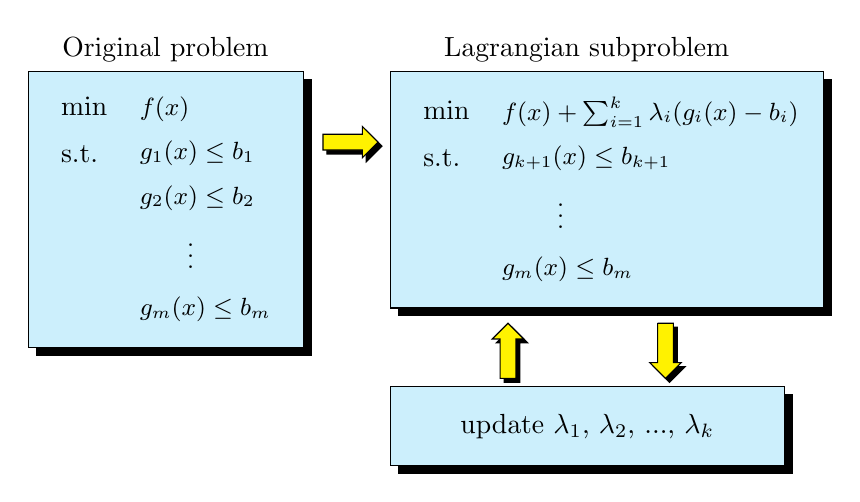
\begin{tikzpicture}

% Box 1 (left) with black shading
\node[below right,draw, minimum width=3.5cm, minimum height=3.5cm, fill=black] at (0.1,-0.1){}; 
\node[below right,draw, minimum width=3.5cm, minimum height=3.5cm, fill=cyan!20] at (0,0){} ;
\node[above] at (1.75,0){Original problem};

% Box 1 left text
\node[below right, text width=3cm] at (0.3,-.2){$\min$\\[5pt] s.t.} ;
\node[below right, text width=3cm, align=left] at (1.3,-.2){\small $f(x)$ \\[5pt] $g_1(x)\leq b_1$ \\[5pt] $g_2(x)\leq b_2$ \\[5pt] \hspace{0.6cm}$\vdots$ \\[5pt] $g_m(x)\leq b_m$};

% Yellow arrow with black shading
\draw[fill =black] (3.8,-1.05) -- ++(0,0.2) -- ++(.5,0) -- ++(0,0.1) -- ++(0.2,-0.2) -- ++(-0.2,-0.2) -- ++(0,0.1) -- cycle;
\draw[fill =yellow] (3.75,-1) -- ++(0,0.2) -- ++(.5,0) -- ++(0,0.1) -- ++(0.2,-0.2) -- ++(-0.2,-0.2) -- ++(0,0.1) -- cycle;

% Box 2 right Top with black shading
\node[below right,draw, minimum width=5.5cm, minimum height=3cm, fill=black] at (4.7,-0.1){};
\node[below right,draw, minimum width=5.5 cm, minimum height=3cm, fill=cyan!20] at (4.6,0){} ;
\node[above] at (7.1,0){Lagrangian subproblem};

% Box 2 text
\node[below right, text width=4cm] at (4.9,-.25){$\min$\\[5pt] s.t.} ;
\node[below right, text width=4cm, align=left] at (5.9,-.2){\small $f(x)+\sum_{i=1}^k \lambda_i(g_i(x)-b_i)$ \\[5pt] $g_{k+1}(x) \leq b_{k+1}$ \\[5pt] \hspace{.7cm}$ \vdots$ \\[5pt] $g_m(x)\leq b_m$ };

% Yellow arrows
\begin{scope}[yshift=-1cm]
\draw[fill =black] (8.05,-2.25) -- ++(0.2,0) -- ++(0,-0.5) -- ++(0.1,0) -- ++(-0.2,-0.2) -- ++(-0.2,0.2) -- ++(0.1,0) -- ++(0,0.5) -- cycle;
\draw[fill =yellow] (8,-2.2) -- ++(0.2,0) -- ++(0,-0.5) -- ++(0.1,0) -- ++(-0.2,-0.2) -- ++(-0.2,0.2) -- ++(0.1,0) -- ++(0,0.5) -- cycle;

\draw[fill =black] (6.05,-2.95) -- ++(0.2,0) -- ++(0,0.5) -- ++(0.1,0) -- ++(-0.2,0.2) -- ++(-0.2,-0.2) --++(0.1,0) -- cycle;

\draw[fill =yellow] (6,-2.9) -- ++(0.2,0) -- ++(0,0.5) -- ++(0.1,0) -- ++(-0.2,0.2) -- ++(-0.2,-0.2) --++(0.1,0) -- cycle;
\end{scope}
% Box 3 with its shading and text
\begin{scope}[yshift=-4cm]
\node[below right,draw, minimum width=5cm, minimum height=1cm, fill=black] at (4.7,-0.1){};
\node[below right,draw, minimum width=5cm, minimum height=1cm, fill=cyan!20] at (4.6,0){update $\lambda_1$, $\lambda_2$, ..., $\lambda_k$} ;
\end{scope}

\end{tikzpicture}

\end{document}
